
\section{enzymes.xml}

The enzyme file is used to define enzyme composition and their catalytic efficiency.
It defines efficiency constraints in the RBA model.
These constraints ensure that a reaction flux is smaller than
the product of efficiency and concentration of the enzyme catalyzing
the reaction.

\subsection{RBAEnzymes}
\label{sec:rba_enzymes}

The outermost portion of the metabolism file is an instance of class
\rbaenzymes, shown in Figure~\ref{fig:enzymes_doc}.

\begin{figure}
  \centering
  \includegraphics[scale=0.8]{figures/enzymes_doc}
  \caption{XML structure of enzyme document.}
\label{fig:enzymes_doc}
\end{figure}

\rbaenzymes{} has no simple attributes.
It contains excatly one instance of \textbf{ListOfEnzymes} that is used
to store \enzyme{} information.


\subsection{Enzyme}
\label{sec:enzyme}

The \enzyme{} class is used to define enzymes
(Fig.~\ref{fig:enzymes_doc}).

It contains a \machinerycomposition{} that refers to metabolic \species{}
and \macromolecule{}s composing the \enzyme{}.
Note that the composition can be left unspecified.
In this case, the reaction associated with the enzyme is considered spontaneous.

\paragraph{The \textit{id} attribute}
The \textbf{id} attribute is a string defining the identifier of
the enzyme.

\paragraph{The \textit{reaction} attribute}
The \textbf{reaction} attribute must match the identifier of a metabolic
\reaction.
It represents the reaction catalyzed by the enzyme.
This must be a one-to-one mapping.
A \reaction{} can only have one associated \enzyme{}.
If several \enzyme{}s catalyze the same \reaction{},
the \reaction{} must be duplicated.

\paragraph{The \textit{forwardEfficiency} attribute}
The \textbf{forwardEfficiency} attribute must match the identifier of a
parameter (\function{} or \aggregate{}).
It represents the forward catalytic constant.

\paragraph{The \textit{backwardEfficiency} attribute}
The \textbf{backwardEfficiency} attribute must match the identifier of a
parameter (\function{} or \aggregate{}).
It represents the backward catalytic constant
(only applicable if reaction catalyzed by enzyme is reversible).

\paragraph{The \textit{zeroCost} attribute}
The \textbf{zeroCost} attribute is a boolean value.
If set to true, the reaction associated may occur without having to produce
the enzyme.
If set to false or unspecified, an efficiency constraint is created where the
flux through the reaction has to be smaller than the product of enzyme
efficiency and enzyme concentration.
